\iffalse
\chapter{2008}
\author{EE24BTECH11019 - Dwarak A}
\section{xe}
\fi

    %17
    \item In an induction motor the phase-difference, $\phi$, between the voltage applied at the stator terminals and the magnetizing current is
        \begin{enumerate}
            \item $\phi=0\degree$
            \item $0\degree<\phi<90\degree$
            \item $\phi=90\degree$
            \item $90\degree<\phi<180\degree$
        \end{enumerate}
    
    %18
    \item A voltage of $+5V$ is applied (with respect to ground) to both the inputs $V_1$ and $V_2$ of an operational amplifier circuit shown in the figure. $R_1=20k\ohm$ and $R_2=10k\ohm$. The output voltage, $V_o$ is
        \begin{figure}[!ht]
        \centering
        \resizebox{0.4\textwidth}{!}{%
\begin{circuitikz}
\tikzstyle{every node}=[font=\large]
\draw (9.25,13.25) to[R,l={ \large $R_2$}] (11.25,13.25);
\draw (12.75,10.75) node[op amp,scale=1, yscale=-1 ] (opamp2) {};
\draw (opamp2.+) to[short] (11.25,11.25);
\draw (opamp2.-) to[short] (11.25,10.25);
\draw (13.95,10.75) to[short](14.25,10.75);
\draw (8.5,11.25) to[R,l={ \large $R_1$}] (11.25,11.25);
\draw (8.5,10.25) to[R,l={ \large $R_1$}] (11.25,10.25);
\draw (11.25,13.25) to[short] (11.25,11.25);
\draw (9.25,13.25) to (9.25,13) node[ground]{};
\draw (8.5,11.25) to[short, -o] (8.25,11.25) node[left] {$V_1$};
\draw (8.5,10.25) to[short, -o] (8.25,10.25) node[left] {$V_2$};
\draw (14.25,10.75) to[short, -o] (14.75,10.75) node[right] {$V_o$};
\draw (11.25,8.75) to[R,l={ \large $R_2$}] (13.75,8.75);
\draw (11.25,10.25) to[short] (11.25,8.75);
\draw (13.75,10.75) to[short] (13.75,8.75);
\end{circuitikz}
}%
        \end{figure}
        \begin{enumerate}
            \item $-5V$
            \item $0V$
            \item $5V$
            \item $20V$
        \end{enumerate}
    
    %19
    \item A pair of zener diodes each with a forward drop of $0.7V$ and a zener voltage of $4.7V$ is connected as shown in the figure. The input voltage is $v_{in}=10sin(2t)$. The peak-to-peak output voltage, $v_o$, is
        \begin{figure}[!ht]
        \centering
        \resizebox{0.4\textwidth}{!}{
\begin{circuitikz}
\tikzstyle{every node}=[font=\large]
\draw (6.5,13.75) to[sinusoidal voltage source, sources/symbol/rotate=auto,l={$V_{in}$}] (6.5,11.75);
\draw (7.25,13.75) to[R,l={$R_S$}] (9.5,13.75);
\draw (10.5,11.75) to[empty Zener diode] (10.5,13.75);
\draw (11.5,13.75) to[empty Zener diode] (11.5,11.75);
\draw (11.5,13.75) to[short, -o] (12.75,13.75) ;
\draw (11.5,11.75) to[short, -o] (12.75,11.75) ;
\draw (9.5,13.75) to[short] (11.5,13.75);
\draw (6.5,13.75) to[short] (7.25,13.75);
\draw (6.5,11.75) to[short] (11.5,11.75);
\node [font=\large] at (12.75,12.75) {$V_o$};
\end{circuitikz}
}
        \end{figure}
        \begin{enumerate}
            \item $5.4V$
            \item $4.7V$
            \item $1.4V$
            \item $0.7V$
        \end{enumerate}

    %20
    \item The npn transistor shown in figure has $h_{fe}=99$ and $V_{BE}=0.7V$. Under quiescent condition, $V_{EG}=4.3V$ and $I_{E}=1mA$, and the current in $R_2$ is $0.1 mA$. The value of $R_1$, required for biasing the circuit is
        \begin{figure}[!ht]
        \centering
        \resizebox{0.25\textwidth}{!}{
\begin{circuitikz}
\tikzstyle{every node}=[font=\large]
\draw (13,14) to[Tnpn, transistors/scale=1.19] (13,16.5);
\draw (13,15.75) node[right] {$C$};
\draw (12.25,15.25) node[above] {$B$};
\draw (13,14.75) node[right] {$E$};
\draw (10.5,16.5) to[R,l={$R_2$}] (10.5,18);
\draw (10.5,14) to[R,l={$R_2$}] (10.5,12.5);
\draw (13,16.5) to[R,l={$R_C$}] (13,18);
\draw (13,14) to[R,l={$R_E$}] (13,12.5);
\draw (10.5,12.5) to[short] (13,12.5);
\draw (10.5,18) to[short] (13,18);
\draw (11.75,18) to[short, -o] (11.75,18.5) node[right] {$15V$};
\draw (11.75,12.5) to (11.75,12) node[ground]{} node[right] {$G$};
\draw (10.5,16.5) to[short] (10.5,14);
\draw (12,15.25) to[short] (10.5,15.25);
\draw[->] (12.5,14) -- (12.5,13) node[midway,left] {$I_E$};
\end{circuitikz}
}
        \end{figure}
        \begin{enumerate}
            \item $10.1k\ohm$
            \item $90.9k\ohm$
            \item $100.1k\ohm$
            \item $150.2k\ohm$
        \end{enumerate}

    %21
    \item The forward characteristics of a p-n diode is given by $i=I_{s}e^{\frac{v}{\brak{nV_{T}}}}$ with $n=2$ and $V_{T}=25mV$. If the diode current is measured to be $100mA$ at $0.7V$ drop, the diode power dissipation at a diode current of $200mA$ is 
        \begin{enumerate}
            \item $70mW$
            \item $140mW$
            \item $143mW$
            \item $147mW$
        \end{enumerate}

    %22
    \item For the n-channel JFET shown in the figure the pinch-off voltage, $V_{p}=-5V$, and gate source voltage, $V_{GS}=-3V$. The minimum required drain to source voltage, $V_{DS}$ to operate at pinch-off condition is
        \begin{figure}[!ht]
        \centering
        \resizebox{0.4\textwidth}{!}{
\begin{circuitikz}
\tikzstyle{every node}=[font=\normalsize]
\draw [ line width=0.2pt ] (9.5,12.5) rectangle (11.5,10);
\draw [line width=0.2pt, short] (9.5,12.25) -- (10,12.25);
\draw [line width=0.2pt, short] (10,12.25) -- (10,10.25);
\draw [line width=0.2pt, short] (10,10.25) -- (9.5,10.25);
\draw [line width=0.2pt, short] (11.5,12.25) -- (11,12.25);
\draw [line width=0.2pt, short] (11,12.25) -- (11,10.25);
\draw [line width=0.2pt, short] (11,10.25) -- (11.5,10.25);
\draw [line width=0.2pt, short] (9.5,12) -- (9.4,12);
\draw [line width=0.2pt, short] (9.4,12) -- (9.4,10.5);
\draw [line width=0.2pt, short] (9.4,10.5) -- (9.5,10.5);
\draw [line width=0.2pt, short] (11.5,12) -- (11.6,12);
\draw [line width=0.2pt, short] (11.6,12) -- (11.6,10.5);
\draw [line width=0.2pt, short] (11.6,10.5) -- (11.5,10.5);
\draw [line width=0.2pt, short] (9.75,12.5) -- (9.75,12.6);
\draw [line width=0.2pt, short] (9.75,12.6) -- (11.25,12.6);
\draw [line width=0.2pt, short] (11.25,12.6) -- (11.25,12.5);
\draw [line width=0.2pt, short] (9.75,10) -- (9.75,9.9);
\draw [line width=0.2pt, short] (9.75,9.9) -- (11.25,9.9);
\draw [line width=0.2pt, short] (11.25,9.9) -- (11.25,10);
\draw (7.25,10.25) to[battery1] (7.25,9.5) node[left] {$V_{GS}$};
\draw [ line width=0.2pt](7.25,10.25) to[short] (7.25,11.25);
\draw [ line width=0.2pt](7.25,11.25) to[short] (9.4,11.25);
\draw [ line width=0.2pt](7.25,9.5) to[short] (7.25,9);
\draw [line width=0.2pt] (10.5,9) to[out=0,in=180] (9.25,9) to[crossing] (7.25,9);
\draw [ line width=0.2pt](10.5,9.9) to[short] (10.5,9);
\draw [ line width=0.2pt](8.25,11.25) to[short] (8.25,8.25);
\draw [ line width=0.2pt](11.6,11.25) to[short] (12.5,11.25);
\draw [ line width=0.2pt](12.5,11.25) to[short] (12.5,8.25);
\draw [ line width=0.2pt](12.5,8.25) to[short] (8.25,8.25);
\draw [ line width=0.2pt](10.5,12.6) to[short, -o] (10.5,13.25) node[right] {$V_D$};
\node at (8.25,11.25) [circ]{};
\node at (8.25, 11.5) {$V_G$};
\draw [ line width=0.2pt](10.5,13.25) to[short] (10.5,13.25);
\node at (10.5,9) [circ]{};
\node at (10.75,9) {$V_S$};
\node at (10.5, 12) {n};
\node at (11.25, 11.25) {p};
\node at (9.75, 11.25) {p};
\end{circuitikz}
}
        \end{figure}
        \begin{enumerate}
            \item $0V$
            \item $2V$
            \item $5V$
            \item $8V$
        \end{enumerate}

    %23
    \item The Boolean function corresponding to the truth table shown is
        \begin{table}[!ht]
        \centering
        \begin{tabular}{c|c|c|c}
    A & B & C & F \\
    \hline
    0 & 0 & 0 & 1 \\
    \hline
    0 & 0 & 1 & 1 \\
    \hline
    0 & 1 & 0 & 0 \\
    \hline
    0 & 1 & 1 & 1 \\
    \hline
    1 & 0 & 0 & 0 \\
    \hline
    1 & 0 & 1 & 1 \\
    \hline
    1 & 1 & 0 & 0 \\
    \hline
    1 & 1 & 1 & 0 \\
    \hline
\end{tabular}
        \end{table}
        \begin{enumerate}
            \item $F=A\overline{B}C+\overline{A}BC+\overline{AB}C+\overline{ABC}$
            \item $F=ABC+AB\overline{C}+\overline{A}BC$
            \item $F=ABC+AB\overline{C}+A\overline{BC}+\overline{A}B\overline{C}$
            \item $F=A\overline{B}C+\overline{A}BC+\overline{AB}C+\overline{A}BC$
        \end{enumerate}

    %24
    \item The decimal number $328$ when converted to the base of $9$ is equivalent to 
        \begin{enumerate}
            \item $(434)_9$
            \item $(424)_9$
            \item $(404)_9$
            \item $(304)_9$
        \end{enumerate}

    %25
    \item The following logic circuit can be represented by the Boolean expression
        \begin{figure}[!ht]
        \centering
        \resizebox{0.6\textwidth}{!}{%
\begin{circuitikz}
\tikzstyle{every node}=[font=\normalsize]
\draw (8,11.25) to[short] (8.25,11.25);
\draw (8,10.75) to[short] (8.25,10.75);
\draw (8.25,11.25) node[ieeestd nor port, anchor=in 1, scale=0.89](port){} (port.out) to[short] (10,11);
\draw (8,8.75) to[short] (8.25,8.75);
\draw (8,8.25) to[short] (8.25,8.25);
\draw (8.25,8.75) node[ieeestd and port, anchor=in 1, scale=0.89](port){} (port.out) to[short] (10,8.5);
\draw (11,11) to[short] (11.25,11);
\draw (11,10.5) to[short] (11.25,10.5);
\draw (11.25,11) node[ieeestd xnor port, anchor=in 1, scale=0.89](port){} (port.out) to[short] (13,10.75);
\draw (11.25,8.5) node[ieeestd not port, anchor=in](port){} (port.out) to[short] (13,8.5);
\draw (port.in) to[short] (11,8.5);
\draw (14.5,10) to[short] (14.75,10);
\draw (14.5,9.5) to[short] (14.75,9.5);
\draw (14.75,10) node[ieeestd or port, anchor=in 1, scale=0.89](port){} (port.out) to[short] (16.5,9.75);
\draw [ line width=0.2pt](10,11) to[short] (11,11);
\draw [ line width=0.2pt](13,10.75) to[short] (13.75,10.75);
\draw [ line width=0.2pt](13.75,10.75) to[short] (13.75,10);
\draw [ line width=0.2pt](13.75,10) to[short] (14.5,10);
\draw [ line width=0.2pt](13,8.5) to[short] (13.75,8.5);
\draw [ line width=0.2pt](13.75,8.5) to[short] (13.75,9.5);
\draw [ line width=0.2pt](13.75,9.5) to[short] (14.5,9.5);
\draw [ line width=0.2pt](10,8.5) to[short] (11,8.5);
\draw [ line width=0.2pt](11,10.5) to[short] (10.5,10.5);
\draw [ line width=0.2pt](10.5,10.5) to[short] (10.5,8.5);
\draw [ line width=0.2pt](8,11.25) to[short] (6.25,11.25);
\draw [ line width=0.2pt](8,8.25) to[short] (6.25,8.25);
\draw [ line width=0.2pt](8,8.75) to[short] (7.5,8.75);
\draw [ line width=0.2pt](8,10.75) to[short] (6.25,10.75);
\draw [ line width=0.2pt](7.5,10.75) to[short] (7.5,8.75);
\node [font=\normalsize] at (17,9.75) {$F$};
\node [font=\normalsize] at (6,11.25) {$A$};
\node [font=\normalsize] at (6,10.75) {$B$};
\node [font=\normalsize] at (6,8.25) {$C$};
\end{circuitikz}
}
        \end{figure}
        \begin{enumerate}
            \item $F=\overline{B}+BC+\overline{C}$
            \item $F=\overline{B}+\overline{C}$
            \item $F=\brak{\overline{B+C}}$
            \item $F=\overline{A}+\overline{B}+\overline{C}$
        \end{enumerate}

    %26
    \item A $4$-bit resistor network based D/A converter is shown in the figure. The output corresponding to the number $1010$ is
        \begin{figure}[!ht]
        \centering
        \resizebox{0.6\textwidth}{!}{%
\begin{circuitikz}
\tikzstyle{every node}=[font=\large]
\draw [line width=0.2pt](8.75,10) to[R] (8.75,12.5) node[right] {$10k\Omega$};
\draw [line width=0.2pt](10.5,10) to[R] (10.5,12.5) node[right] {$20k\Omega$};
\draw [line width=0.2pt](12.5,10) to[R] (12.5,12.5) node[right] {$40k\Omega$};
\draw [line width=0.2pt](14.25,10) to[R] (14.25,12.5) node[right] {$80k\Omega$};
\draw [line width=0.2pt](8.75,15) to[normal open switch] (8.75,12.5);
\draw [line width=0.2pt](10.5,15) to[normal open switch] (10.5,12.5);
\draw [line width=0.2pt](12.5,15) to[normal open switch] (12.5,12.5);
\draw [line width=0.2pt](14.25,15) to[normal open switch] (14.25,12.5);
\draw [ line width=0.2pt](14.25,15) to[short] (6.25,15);
\draw (6.25,15) to[battery1] (6.25,11.25);
\draw [line width=0.2pt](6.25,11.25) to (6.25,10.25) node[ground]{};
\draw [ line width=0.2pt](8.75,10) to[short] (16.25,10);
\draw [ line width=0.2pt](17.75,9.5) node[op amp,scale=1] (opamp2) {};
\draw [ line width=0.2pt](opamp2.+) to[short] (16.25,9);
\draw [ line width=0.2pt] (opamp2.-) to[short] (16.25,10);
\draw [ line width=0.2pt](18.95,9.5) to[short](19.25,9.5);
\draw [line width=0.2pt](16.25,9) to (16.25,8) node[ground]{};
\draw [ line width=0.2pt](19.25,9.5) to[short, -o] (21.25,9.5) node[right] {$V_o$};
\draw [ line width=0.2pt](16.25,11.75) to[R, l=$5k\Omega$] (18.75,11.75);
\draw [ line width=0.2pt](16.25,11.75) to[short] (16.25,10);
\draw [ line width=0.2pt](18.75,11.75) to[short] (18.75,9.5);
\end{circuitikz}
}

        \end{figure}
        \begin{enumerate}
            \item $5.0V$
            \item $6.25V$
            \item $7.25V$
            \item $10.0V$
        \end{enumerate}

    %27
    \item Two $10V$ square waves of same frequency but $90\degree$ out-of-phase to each other are applied to $X$ and $Y$ deflecting plates of a CRO. Both channels are set at $5V$/division and the CRO is operating in the $X-Y$ mode. The display on CRO will be 
        \begin{enumerate}
            \item A bright circle
            \item A bright ellipse
            \item Two bright spots at the diagonal of a faint square
            \item Four bright spots at the comers of a faint square
        \end{enumerate}

    %28
    \item CRO that is used in $X-Y$ mode displays a line inclined at an angle of $135\degree$. The $X$-channel gain is $5V$/division and the $Y$-channel gain is $10V$/division. If the display point at a given instant corresponds to $+3$ divisions on the $X$-axis, the input voltage to the $Y$-channel at that instant is 
        \begin{enumerate}
            \item $-30V$
            \item $-15V$
            \item $+15V$
            \item $+30V$
        \end{enumerate}

%\subsection*{Common Data Questions}

Common Data for Questions 29 and 30:

A $1.0kW$ induction motor has $15$ pole-pairs and is supplied from a $60Hz$ source. The motor runs at $0.05$ slip. The stator loss is $80W$.
    
    %29
    \item The speed of the rotating magnetic field in the motor and the frequency of the rotor induced voltage are
        \begin{enumerate}
            \item $120rpm, 1.5Hz$
            \item $120rpm, 28.5Hz$
            \item $240rpm, 3.0Hz$
            \item $240rpm, 57.0Hz$
        \end{enumerate}

    %30
    \item The rotor copper loss of this induction motor is
        \begin{enumerate}
            \item $120rpm, 1.5Hz$
            \item $120rpm, 28.5Hz$
            \item $240rpm, 3.0Hz$
            \item $240rpm, 57.0Hz$
        \end{enumerate}

%\subsection*{Linked Answer Questions: Q.31 to Q.34 carry two marks each.}

Statement for Linked Answer Questions 31 and 32:

A practical dc voltage source is represented as an ideal dc voltage source in series with an internal resistance. The $V-I$ characteristics of two such sources, $E_1$ and $E_2$, are shown in the figure.
        \begin{figure}[!ht]
        \centering
        \resizebox{0.5\textwidth}{!}{%
\begin{circuitikz}
\tikzstyle{every node}=[font=\large]
\draw [->, >=Stealth] (8.75,8.75) -- (8.75,15.75);
\draw [->, >=Stealth] (8.75,8.75) -- (17.5,8.75);
\draw [dashed] (16.25,8.75) -- (16.25,13.75);
\draw [short] (8.75,13.75) -- (16.25,13.25)node[pos=0.5,below]{$E_2$};
\draw [short] (8.75,15) -- (16.25,13.75)node[pos=0.5,above]{$E_1$};
\node [font=\large] at (8,15) {$100V$};
\node [font=\large] at (8,13.5) {$80V$};
\node [font=\large] at (16.75,13.75) {$80V$};
\node [font=\large] at (16.75,13.25) {$72V$};
\node [font=\large] at (8.75,8.5) {$0A$};
\node [font=\large] at (12.5,8.25) {Current};
\node [font=\large] at (7.5,11.75) {Voltage};
\node [font=\large] at (16.25,8.5) {$4A$};
\draw[domain=8.25:9.25,samples=100,smooth] plot (\x,{0.15*sin(6.3*\x r -8.25 r ) +10});
\draw[domain=8.25:9.25,samples=100,smooth] plot (\x,{0.15*sin(6.3*\x r -8.25 r ) +9.75});
\end{circuitikz}
}
        \end{figure}

    %31
    \item The respective internal resistances of $E_1$ and $E_2$ are
        \begin{enumerate}
            \item $20\ohm,8\ohm$
            \item $5\ohm,2\ohm$
            \item $8\ohm,20\ohm$
            \item $2\ohm,5\ohm$
        \end{enumerate}

    %32
    \item If the two sources, $E_1$ and $E_2$, in question Q.31 are connected in parallel to feed a load of $200\ohm$ resistance, then the load current is in the range 
        \begin{enumerate}
            \item $0.0A$ to $0.5A$
            \item $0.5A$ to $2.0A$
            \item $2.0A$ to $4.0A$
            \item $4.0A$ to $8.0A$
        \end{enumerate}

Statement for Linked Answer Questions 33 and 34:

A function $F$, in "Sum of Product (SOP)" form is described by $$F=\sum m(0,1,3,4,5,6,7,13,15)$$

    %33
    \item The Karnaugh Map for $F$ is given by ($X$ being don't care)
        \begin{enumerate}
            \item $$
                \begin{array}{|c|c|c|c|c|}
                \hline
                    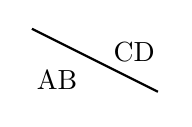
\begin{tikzpicture}
        \node at (0.1,0.1) {CD};
        \draw[thick] (0.4,-0.4) -- (-1.2,0.4);
        \node[anchor=south east] at (-0.5,-0.5) {AB};
    \end{tikzpicture}
                & 00 & 01 & 11 & 10 \\
                \hline
                00 & X & X & X & 1 \\
                \hline
                01 & X & X & X & X \\
                \hline
                11 & 1 & X & X & 1 \\
                \hline
                10 & 1 & 1 & 1 & 1 \\
                \hline
            \end{array}
            $$
            \item $$
                \begin{array}{|c|c|c|c|c|}
                \hline
                    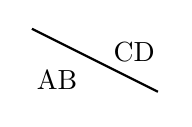
\begin{tikzpicture}
        \node at (0.1,0.1) {CD};
        \draw[thick] (0.4,-0.4) -- (-1.2,0.4);
        \node[anchor=south east] at (-0.5,-0.5) {AB};
    \end{tikzpicture}
                & 00 & 01 & 11 & 10 \\
                \hline
                00 & 1 & 1 & 1 & X \\
                \hline
                01 & 1 & 1 & 1 & 1 \\
                \hline
                11 & X & 1 & 1 & x \\
                \hline
                10 & X & X & X & X \\
                \hline
            \end{array}
            $$
            \item $$
                \begin{array}{|c|c|c|c|c|}
                \hline
                    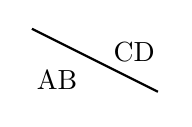
\begin{tikzpicture}
        \node at (0.1,0.1) {CD};
        \draw[thick] (0.4,-0.4) -- (-1.2,0.4);
        \node[anchor=south east] at (-0.5,-0.5) {AB};
    \end{tikzpicture}
                & 00 & 01 & 11 & 10 \\
                \hline
                00 & 1 & X & 1 & X \\
                \hline
                01 & X & 1 & X & 1 \\
                \hline
                11 & 1 & X & X & X \\
                \hline
                10 & X & 1 & X & 1 \\
                \hline
            \end{array}
            $$
            \item $$
                \begin{array}{|c|c|c|c|c|}
                \hline
                    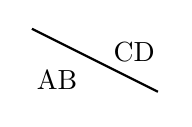
\begin{tikzpicture}
        \node at (0.1,0.1) {CD};
        \draw[thick] (0.4,-0.4) -- (-1.2,0.4);
        \node[anchor=south east] at (-0.5,-0.5) {AB};
    \end{tikzpicture}
                & 00 & 01 & 11 & 10 \\
                \hline
                00 & 1 & 1 & X & X \\
                \hline
                01 & X & X & X & X \\
                \hline
                11 & X & 1 & 1 & 1 \\
                \hline
                10 & X & 1 & 1 & X \\
                \hline
            \end{array}
            $$
        \end{enumerate}

    %34
    \item Using the Karnaugh Map obtained in question Q.33, the function, $F$ reduces to 
        \begin{enumerate}
            \item $F=\overline{AC}+\overline{A}D+AB+BD$
            \item $F=AC+AD+\overline{AB}+\overline{BD}$
            \item $F=AC+\overline{A}D+\overline{AB}+\overline{BD}$
            \item $F=\overline{AC}+\overline{A}D+\overline{A}B+BD$
        \end{enumerate}

